
\renewcommand{\arraystretch}{1.5} % Default value: 1

%%% Write here
%%%%%%%%%%%%%%%%%%%%%%%%%%%%%%%%%%%%%
\section{Introduction}
The Fabry-Perot interferometer is an important optical instrument used for high-resolution interference and spectroscopic measurements. This interferometer, designed in 1899 by C. Fabry and A. Perot, represents a significant improvement over the Michelson interferometer. It contains plane surfaces that are all partially reflecting so that multiple rays of light are responsible for creation of the observed interference patterns. The Fabry-Perot model still follows the general principle of interferometry, but the resulting fringes are considerably more clearly defined because of the many reflections that highlight the regions where constructive and destructive effects take place.
%%%%%%%%%%%%%%%%%%%%%%%%%%%%%%%%%%%%%
\section{Objective}
This experiment has two parts: 
\subsubsection*{Part A}
\begin{enumerate}
    \item Observe circular interference fringes produced by a Fabry-Perot interferometer using a monochromatic laser source.
    \item Using a known wavelength laser source we have to find the spacing between two plane surfaces in the Fabry-Perot interferometer.
    \item Using the calculated spacing information we have to find a unknown wavelength of a laser.
    \item We have to find finesse, free spectral range (FSR), contrast of the Etalon.
\end{enumerate}
\subsubsection*{Part B}
\begin{enumerate}
    \item We have to analysis the image of fringes using ImageJ software.
    \item Then useful parameters need to found based on the calculation from the fitting.
\end{enumerate}

%%%%%%%%%%%%%%%%%%%%%%%%%%%%%%%%%%%%%
\section{Equipment Required}
The following equipments are required to perform this experiment, 
\begin{itemize}
    \item Diode lasers (green and red) with with power supply
    \item Convex lens 
    \item Fabry-Perot interferometer
    \item Optical mounts and translation stage
    \item Screen for observing interference fringes
\end{itemize}
%%%%%%%%%%%%%%%%%%%%%%%%%%%%%%%%%%%%%
\section{Theory}
The Fabry-Perot interferometer consists of two parallel, partially reflecting plane mirrors separated by a distance d, forming an optical resonant cavity. When monochromatic light enters the cavity, multiple reflections occur between the mirrors, producing multiple beam interference. Constructive interference occurs only for specific angles and wavelengths that satisfy the resonance condition. For a given spacing $L_1$ the interferometer will transmit only certain wavelengths $\lambda$ as determined by

\begin{equation}
\label{eq:airy_profile}
T = \frac{\tau_0}{1 + \frac{4F^2}{\pi^2}
\sin^2\!\left( \frac{2\pi L_1}{\lambda} \right)}
\end{equation}
where $\tau_0$ (<1) is the maximum possible transmission determined by losses in the system, and F, the finesse, is a quality factor depending primarily on the mirror reflectivity and flatness. This equation shows that only those wavelengths satisfying
\begin{equation}
    L_1 = \frac{1}{2} p\lambda
\end{equation}
for integral values of p, will be transmitted.

\begin{figure}
    \centering
    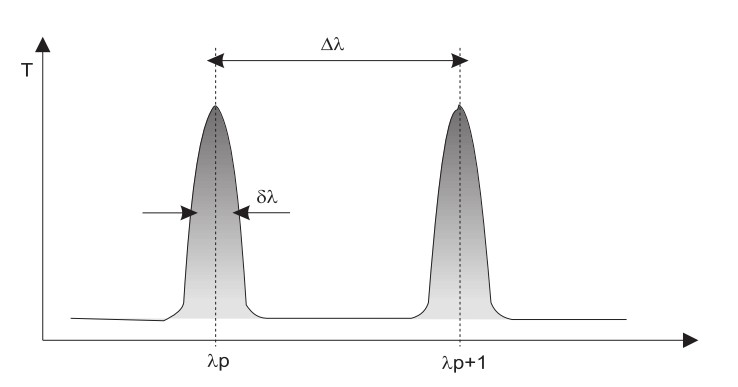
\includegraphics[width = 0.8\textwidth]{Image/Fig5.jpg}
    \caption{Variation of transmitance over wavelength}
\end{figure}
\subsection{Relation between the radius of the fringe and the order of the fringe}
In a Fabry--Perot interferometer, the condition for \textbf{constructive interference} is
\begin{equation}
m\lambda = 2d\cos\theta ,
\end{equation}
where $m$ is the order of interference, $d$ is the separation between the plates, $\lambda$ is the wavelength of light, and $\theta$ is the angle of emergence. As $\theta$ increases, the order $m$ decreases, and hence the order of the rings decreases with increasing radius. The integer nearest to $2d/\lambda$ corresponds to the order of the fringe system at the centre.

For the $m^{\text{th}}$ ring,
\begin{equation}
m\lambda = 2d\cos\theta_m .
\end{equation}

For successive rings,
\begin{align}
(m+1)\lambda &= 2d\cos\theta_{m+1}, \\
(m+2)\lambda &= 2d\cos\theta_{m+2}, \\
(m+3)\lambda &= 2d\cos\theta_{m+3}, \\
&\vdots
\end{align}

Subtracting the above equations from that of the $m^{\text{th}}$ ring, we obtain
\begin{align}
\lambda &= 2d\left( \cos\theta_m - \cos\theta_{m+1} \right), \\
2\lambda &= 2d\left( \cos\theta_m - \cos\theta_{m+2} \right), \\
3\lambda &= 2d\left( \cos\theta_m - \cos\theta_{m+3} \right), \\
&\vdots \\
n\lambda &= 2d\left( \cos\theta_m - \cos\theta_{m+n} \right).
\end{align}

Hence,
\begin{equation}
\label{eq:n_cos_diff}
n = \frac{2d}{\lambda}\left( \cos\theta_m - \cos\theta_{m+n} \right).
\end{equation}

From the geometry of the fringe pattern,
\begin{equation}
\tan\theta_m = \frac{\chi_m}{D},
\end{equation}

where $\chi_m$ is the radius of the $m^{\text{th}}$ fringe and $D$ is the distance between the etalon and the screen.

Hence,
\begin{equation}
\cos^2\theta_m = \frac{1}{1+\tan^2\theta_m}.
\end{equation}

When $D$ is large, $\theta_m$ is small and
\begin{equation}
\theta_m \approx \frac{\chi_m}{D}.
\end{equation}

Therefore,
\begin{equation}
\cos^2\theta_m = \frac{1}{1+\left(\frac{\chi_m^2}{D^2}\right)},
\end{equation}

and
\begin{equation}
\cos\theta_m = \left[ 1+\left(\frac{\chi_m^2}{D^2}\right) \right]^{-1/2}.
\end{equation}

Using the binomial approximation for small $\frac{\chi_m^2}{D^2}$,
\begin{equation}
\cos\theta_m \approx 1 - \frac{\chi_m^2}{2D^2}.
\end{equation}

Substituting this into the relation \cref{eq:n_cos_diff}, we obtain

\begin{align}
n &= \frac{2d}{\lambda}
\left[
\left(1 - \frac{\chi_m^2}{2D^2}\right)
-
\left(1 - \frac{\chi_{m+n}^2}{2D^2}\right)
\right], \\
&= \frac{2d}{\lambda}\left( \frac{\chi_{m+n}^2 - \chi_m^2}{2D^2} \right).
\end{align}

Hence,
\begin{equation}
\boxed{n = \frac{d}{\lambda D^2}
\left( \chi_{m+n}^2 - \chi_m^2 \right)}.
\end{equation}

Defining
\begin{equation}
\chi_n^2 = \chi_{m+n}^2 - \chi_m^2,
\end{equation}

we finally obtain
\begin{equation}
\label{eq:final_eq}
\boxed{n = \frac{d}{\lambda D^2}\, \chi_n^2}.
\end{equation}

\subsection{Free Spectral Range}
The Free Spectral Range (FSR) of a Fabry-Perot interferometer is the spacing in optical frequency or wavelength between two successive transmission or reflection maxima. It defines the maximum spectral bandwidth that the etalon can filter or measure without causing overlapping interference orders.
\begin{equation}
    \begin{gathered}
        \text{FSR in frequency} = \frac{c}{2d}  \\
        \text{FSR in wavelength} \; \Delta \lambda =  \frac{\lambda^2}{2d} \\ 
        \text{FSR in wavenumber} = \frac{1}{2d}
    \end{gathered}
\end{equation}
\subsection{Finesse}
Finesse (\(F\)) in a Fabry-Perot interferometer is a dimensionless measure of the sharpness of its transmission resonances, defining the ratio of the Free Spectral Range (FSR) to the Full Width at Half Maximum (FWHM) of the fringes. It quantifies how well the device separates closely spaced wavelengths. A high-finesse etalon exhibits narrower, sharper peaks, allowing for higher resolution, and is determined by cavity losses and mirror reflectivity.

\begin{equation}
    \text{F} = \frac{\text{FSR}}{\text{FWHM}} = \frac{\pi\sqrt{R}}{1 - R}
\end{equation}
where \(R\) is the reflectivity of the mirrors.

\subsection{Contrast}
In a Fabry-Perot interferometer, contrast refers to the ratio of the maximum transmitted intensity to the minimum transmitted intensity in the interference pattern. It is a critical figure of merit that defines the device's ability to separate closely spaced spectral components of different intensities.
\begin{equation}
\text{Contrast } (C) = \frac{I_{\max}}{I_{\min}}
= \left( \frac{2F}{\pi} \right)^2 + 1
\end{equation}
where $F$ is the finesse of the Fabrey Perot interferometer.
%%%%%%%%%%%%%%%%%%%%%%%%%%%%%%%%%%%%%
\section{Setup}

\begin{figure}[H]
    \centering
    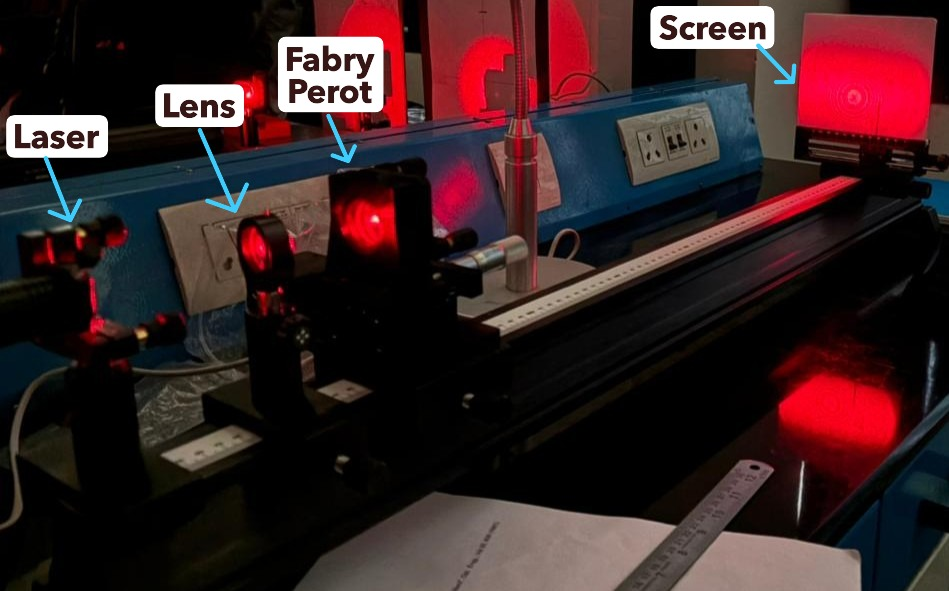
\includegraphics[width = 0.8\textwidth]{Image/Fig2_final.JPG}
    \caption{Setup of Fabry-Perot interferometer}
\end{figure}
The above figure is the step up used in the lab. Here the components are pointed and labeled accordingly. Another schematic of the set up is given below.
\begin{figure}[H]
    \centering
    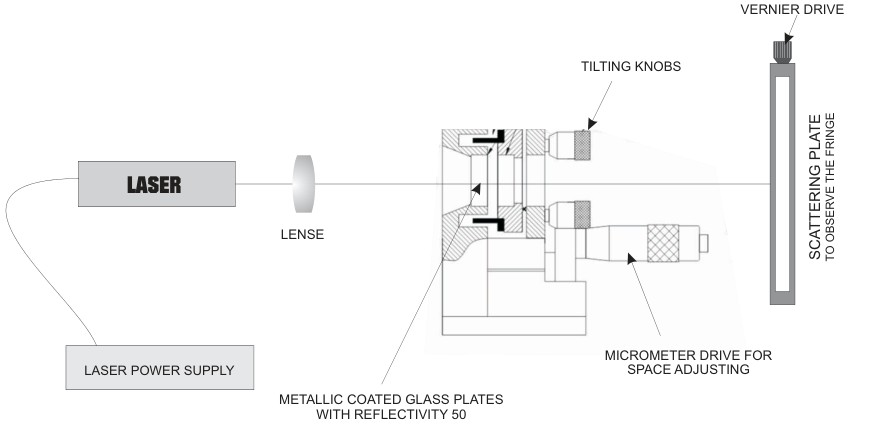
\includegraphics[width = 0.7\textwidth]{Image/Fig3.jpg}
    \caption{Schematic setup of Fabry-Perot interferometer}
\end{figure}
\noindent We used the green and red Diode lasers. And the whole step up is placed on a rail with a scale attached with it. 

%%%%%%%%%%%%%%%%%%%%%%%%%%%%%%%%%%%%%
\section{Data analysis and calculation} 
\subsubsection*{Part A}
For the first part of \textbf{Part A}, green laser is used. The wavelength is known, $\lambda_g = 532\;nm$. The separation between the etalon and the screen (D) is 598 mm.
\begin{center}
\begin{longtable}{|c|c|c|c|c|c|c|}
\caption{Data taken using green laser ($\lambda = 532\;nm$)} \\
\toprule
n & m & left side (mm) & right side (mm) & Diameter (mm) & radius (mm)  & $\chi_n^2 = \chi_{m+n}^2 - \chi_m^2$\\
\endfirsthead
\multicolumn{7}{c}%
    {{\bfseries \tablename\ \thetable{} -- continued from previous page}} \\ \hline
    %
\endhead
\hline \multicolumn{7}{|r|}{{Continued on next page}} \\ \hline
\endfoot
\hline \hline
\endlastfoot
\midrule
%
0 & 1 & 70.7           & 50.6            & 20.1     & 10.05  &       \dots  \\ \hline
1 & 2 & 77.6           & 45.5            & 32.1     & 16.05  & 156.6    \\ \hline
2 & 3 & 81.2           & 40.6            & 40.6     & 20.3   & 311.0875 \\ \hline
3 & 4 & 85             & 36.1            & 48.9     & 24.45  & 496.8    \\ \hline
4 & 5 & 88.4           & 33.8            & 54.6     & 27.3   & 644.2875 \\ \hline
5 & 6 & 91             & 30.9            & 60.1     & 30.05  & 802      \\ \hline
6 & 7 & 94             & 27.5            & 66.5     & 33.25  & 1004.56  \\ \hline
7 & 8 & 97             & 25.1            & 71.9     & 35.95  & 1191.4  \\
\bottomrule
\end{longtable}
\end{center}
Using this data the following plot is done between fringe order (n) and the $\chi_n^2 = \chi_{m+n}^2 - \chi_m^2$. 
\begin{figure}[H]
    \centering
    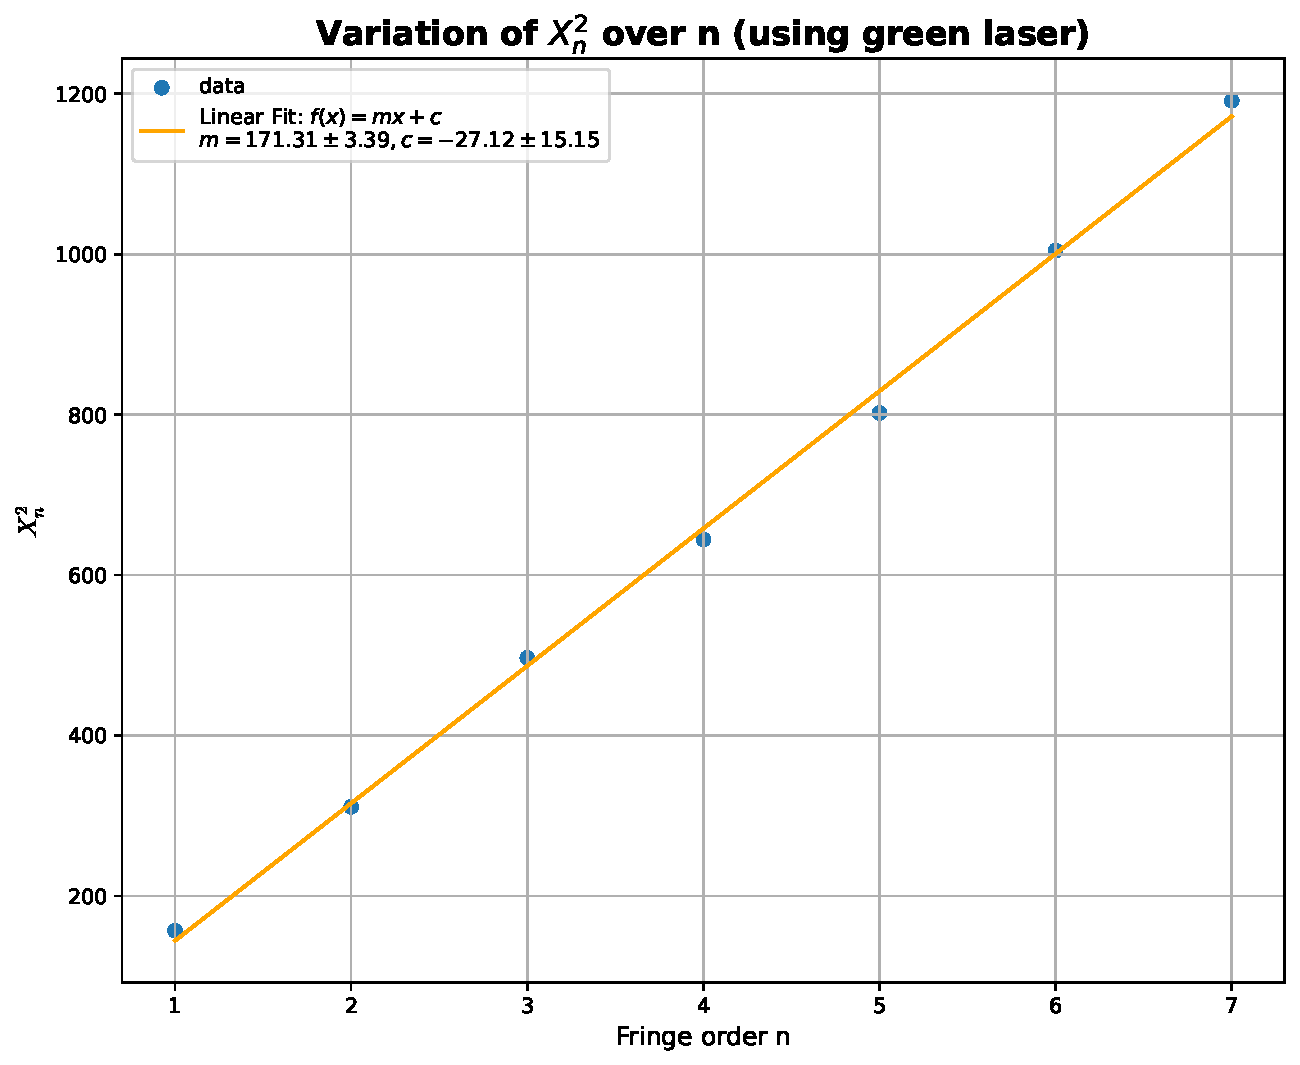
\includegraphics[width=0.8\linewidth,page = 1]{Image/Plot1.pdf}
    \caption{$\chi_n^2$ vs n for green laser}
    \label{fig:plot1}
\end{figure}

The data points are fitted using a straight line. The slope of the straight line is $173.31 \pm 3.39$ and the y intercept is $-27.12 \pm 15.15$. From this and using the equation \cref{eq:final_eq}, we can have the value of d,
\[
d = \frac{\lambda D^2}{\text{slope}} = \frac{{598}^2\times 0.000532 }{173.31} = 1.11\;\text{mm}
\]

Now for the second part, the similar data taken for red laser to find the wavelength of the red laser using the separation of the etalon using same D = 598 mm.
\begin{figure}[H]
    \centering
    \begin{subfigure}[b]{0.45\textwidth}
        \centering
        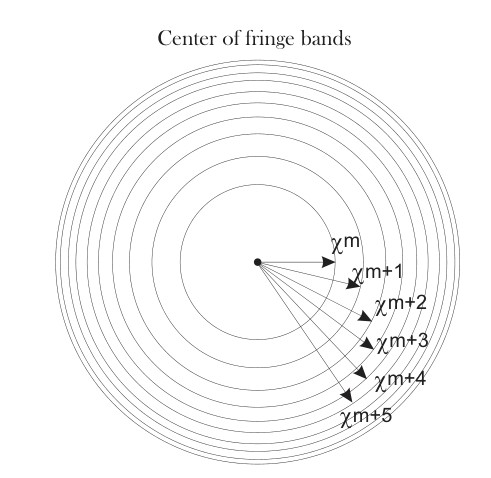
\includegraphics[width = \textwidth]{Image/Fig4.jpg}
        \caption{Line drawing of Fabrey Perot fringe pattern}
    \end{subfigure}
    \hfill
    \begin{subfigure}[b]{0.45\textwidth}
        \centering
        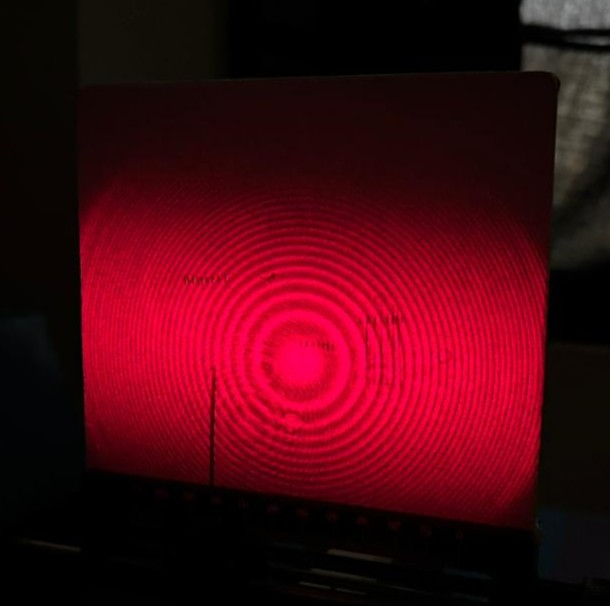
\includegraphics[width = \textwidth]{Image/Fig1.jpeg}
        \caption{Observation of Fabrey Perot fringe pattern}
    \end{subfigure}
    \caption{Fringes in Fabrey Perot interferometer}  
    % \label{fig:enter-label}
\end{figure}

\begin{center}
\begin{longtable}{|c|c|c|c|c|c|c|}
\caption{Data taken using red laser} \\
\toprule
n & m & left side (mm) & right side (mm) & Diameter (mm) & radius (mm)  & $\chi_n^2 = \chi_{m+n}^2 - \chi_m^2$\\
\endfirsthead
\multicolumn{7}{c}%
    {{\bfseries \tablename\ \thetable{} -- continued from previous page}} \\ \hline
    %
\endhead
\hline \multicolumn{7}{|r|}{{Continued on next page}} \\ \hline
\endfoot
\hline \hline
\endlastfoot
\midrule
%
0 & 1 & 70.7           & 50.6            & 20.1     & 10.05  &    \dots  \\ \hline
1 & 2 & 77.6           & 45.5            & 32.1     & 16.05  & 156.6    \\ \hline
2 & 3 & 81.2           & 40.6            & 40.6     & 20.3   & 311.0875 \\ \hline
3 & 4 & 85             & 36.1            & 48.9     & 24.45  & 496.8    \\ \hline
4 & 5 & 88.4           & 33.8            & 54.6     & 27.3   & 644.2875 \\ \hline
5 & 6 & 91             & 30.9            & 60.1     & 30.05  & 802      \\ \hline
6 & 7 & 94             & 27.5            & 66.5     & 33.25  & 1004.56  \\ \hline
7 & 8 & 97             & 25.1            & 71.9     & 35.95  & 1191.4 \\
\bottomrule
\end{longtable}
\end{center}

Using this data the following plot is done between fringe order (n) and the $\chi_n^2 = \chi_{m+n}^2 - \chi_m^2$. 

\begin{figure}[H]
    \centering
    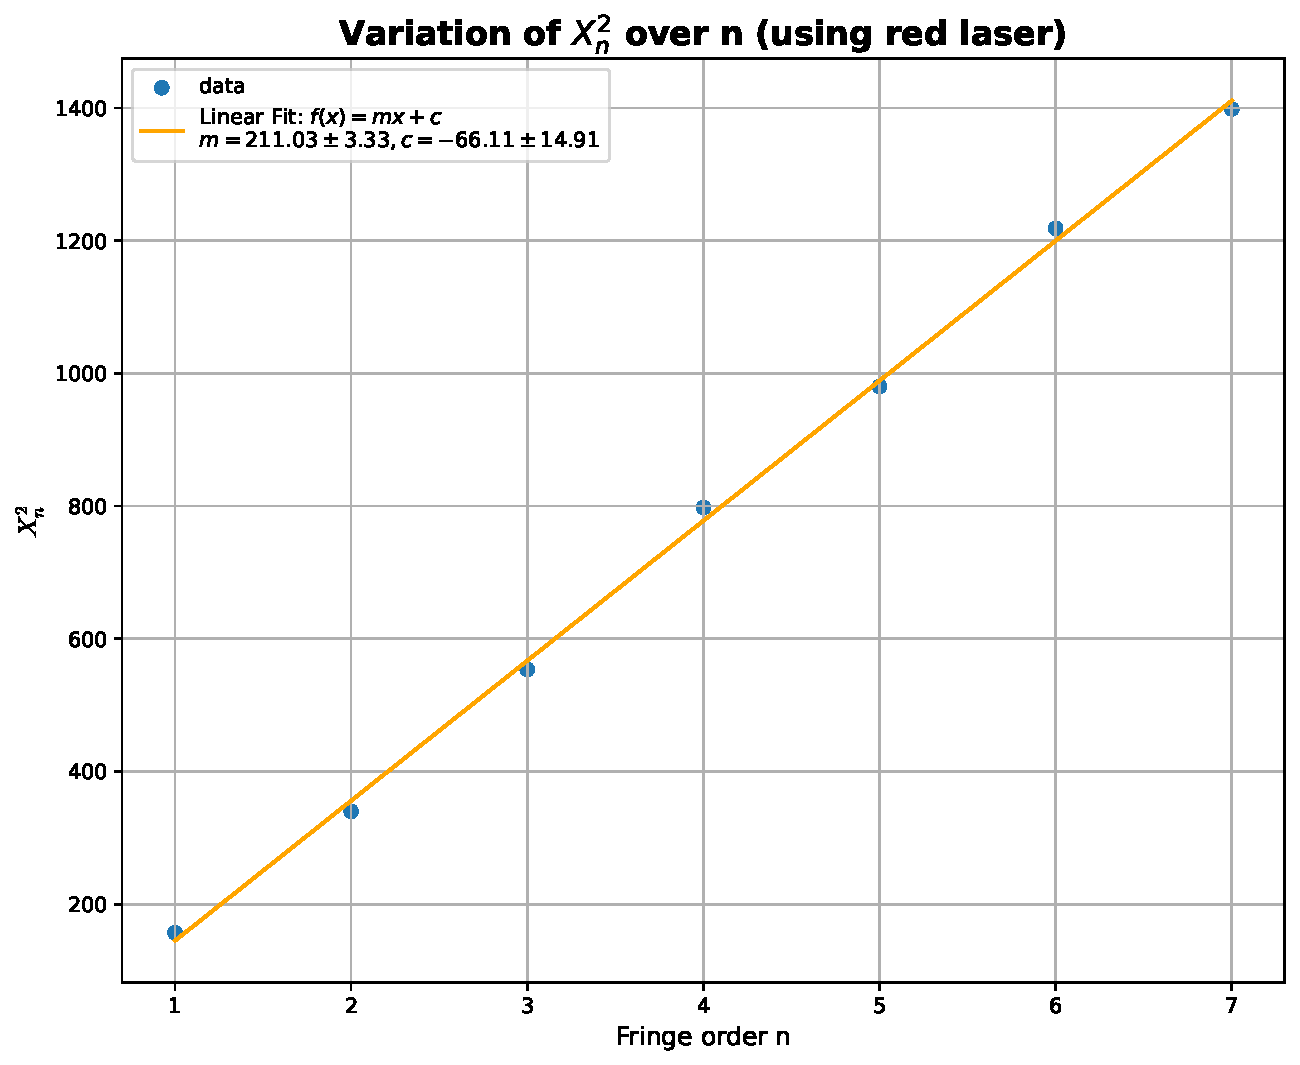
\includegraphics[width=0.8\linewidth,page = 1]{Image/Plot2.pdf}
    \caption{$\chi_n^2$ vs n for red laser}
    \label{fig:plot2}
\end{figure}

The data points are fitted using a straight line. The slope of the straight line is $211.03 \pm 3.33$ and the y intercept is $-66.11 \pm 14.91$. From this and using the equation \cref{eq:final_eq}, we can have the value of $\lambda$ for red laser,
\[
\lambda_{red} = \frac{d \times \text{slope}}{D^2} = \frac{1.11 \times 211.03}{598^2} = 0.000655 \; mm = 655 \; nm
\]

Now, we have used power meter to take the measurements of the intensity of the incident beam and beam passing through the etalon using red laser. \textbf{The power of the incident beam} is 50.9 mW and \textbf{the power of the beam after passing through the etalon} is 5.1 mw. The ratio of this power is 0.1002 which is the \textbf{transmitance}, so the \textbf{reflectance} is (1 - transmitance) or $(1- 0.1002) = 0.8998$.
We can find the Free Spectral Range of the Etalon (FSR) using the following relation,
\[
\text{FSR in frequency} = \frac{c}{2d} = \frac{3 \times 10^8}{2 \times 1.11 \times 10^-3} = 1.35 \times 10^{11} \; \text{Hz} = 135 \; \text{GHz}
\]
\begin{align*}
    \text{FSR in wavelength} \; \Delta \lambda &=  \frac{\lambda^2}{2d} = \frac{(655 \times 10^{-9})^2}{2 \times 1.11 \times 10^-3} = 0.1933\; \text{nm}\; \text{(for red laser)}\\
    &=  \frac{\lambda^2}{2d} = \frac{(532 \times 10^{-9})^2}{2 \times 1.11 \times 10^-3} = 0.1275 \;\text{nm} \; \text{(for green laser)}
\end{align*}
\[
\text{FSR in wavenumber} = \frac{1}{2d} = \frac{1}{2 \times 1.11 \times 10^-3} = 9.01 \times 10^{2}
\]
Hence we can find the finesse,
\[
\text{Finesse (F)} = \frac{\pi\sqrt{R}}{1 - R} = \frac{\pi \times \sqrt{0.8998}}{1-0.8998} = 29.74
\]

Similarly, we can find the FWHM, 
\[
\text{FWHM} = \frac{2(1-R)}{\sqrt{R}} = \frac{2\times(1-0.8998)}{\sqrt{0.8998}} = 0.21
\]

Also, we can find the contrast, 
\[
\text{C} = \left(\frac{2F}{\pi}\right)^2 + 1 = \left(\frac{2\times 29.74}{\pi}\right)^2 + 1 = 359.46
\]

So, from the data analysis of this part we have found the following things
\begin{enumerate}
    \item The separation between the etalon $d = 1.11\;mm$.
    \item The wavelength of the red laser is $\lambda = 655\;nm$.
    \item The FSR in frequency is $135 \; \text{GHz}$.
    \item The FSR in wavelength is $0.1933$ nm (for red laser) and $0.1275$ nm (for green laser).
    \item The FSR in wavenumber is $9.01 \times 10^2$
    \item The Finesse (F) is 29.74.
    \item The FWHM is 0.21.
    \item The Contrast(C) is 359.46.
\end{enumerate}

\subsubsection*{Part B}
For the second part we have taken the image of the fringes by putting the lense infront of the etalon. The fringes are align with the vertical. Then using \textit{ImageJ} software, the image is properly croped, gray scaled (32 bit). Using the software the substruction of the background is done. Now using a rectangualar croped tool the analysis is done. This data is fitted in python with the Airy profile mentioned in the \cref{eq:airy_profile}.

\begin{figure}[H]
    \centering
    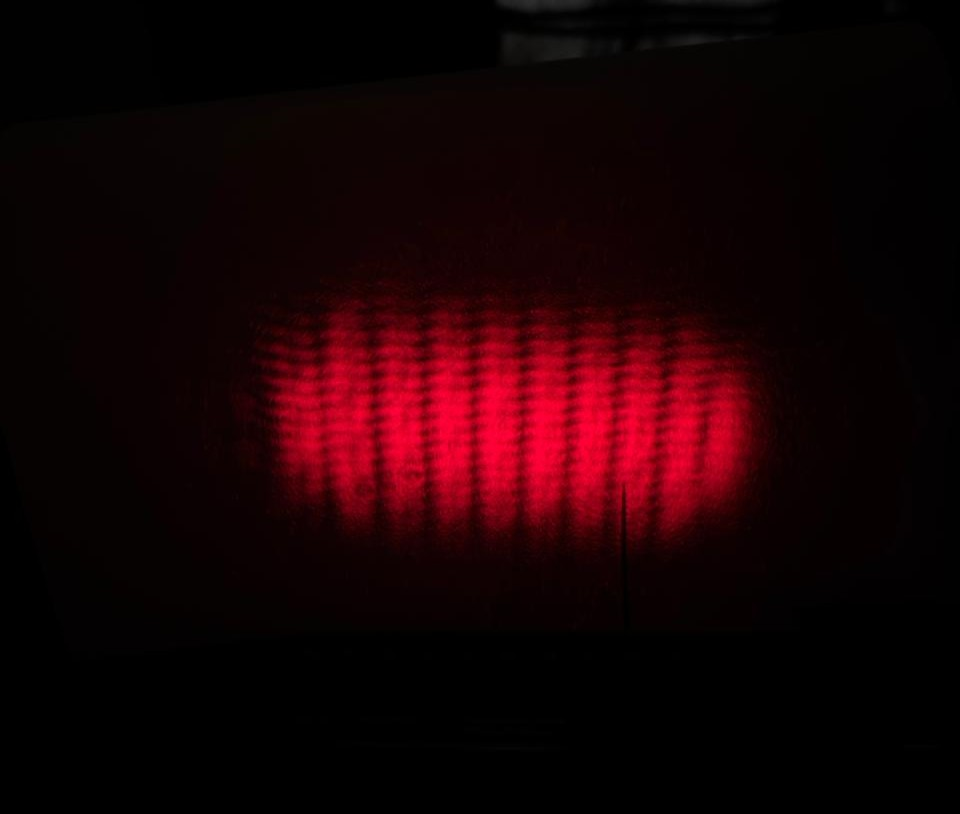
\includegraphics[width = 0.6\textwidth]{Image/Fig_2.jpeg}
    \caption{This is the fringe image used for analysis}    
    \label{fig:fringe_vertical}
\end{figure}  

\noindent This python function is used to fit \textit{Airy profile} with the data set extracted from the above image. Note that the data is normalised. 
\begin{lstlisting}
# normalise intensity
y = y - y.min()
y = y / y.max()

def airy_profile(x, tau0, finesse, alpha, phi):
    return tau0 / (
        1 + (4*finesse**2/np.pi**2) * np.sin(alpha*x + phi)**2
    )
\end{lstlisting}

\begin{figure}[H]
    \centering
    
\includegraphics[width=0.8\linewidth,page = 1]{Image/Plot3.pdf}
    \caption{The fitted Airy profile}
    \label{fig:plot3}
\end{figure}

\noindent From this graph we got the following values of the parameters.
\begin{itemize}
    \item F = 1.97
    \item $\alpha = 0.066$ rad/pixel (which is the conversion factor)
    \item $\tau_0 = 0.91$
    \item $\text{C} = \frac{T_{max}}{T_{min}} = 3.79$
\end{itemize}

\begin{figure}[H]
    \centering
    
\includegraphics[width=0.7\linewidth,page = 1]{Image/Plot4.pdf}
    \caption{The fitted Lorentzian on the central fringe}
    \label{fig:plot4}
\end{figure}
We have fitted the central fringe and got the FWHM to be 92.28 pixel.
%%%%%%%%%%%%%%%%%%%%%%%%%%%%%%%%%%%%
\section{Error Analysis}
\subsection{Fitting Error and progation of error in Part A}
\begin{enumerate}
    \item In the first plot (see \cref{fig:plot1}), the slope is $173.31 \pm 3.39$
    \item In the second plot (see \cref{fig:plot2}), the slope is $211.03 \pm 3.33$
\end{enumerate}
So by using the propagation of error we have,
\subsubsection*{Error in separation}
\[
\frac{\Delta d}{d} = \left|\frac{\Delta \text{slope}}{\text{slope}} \right| + 2\left|\frac{\Delta D}{D} \right|= \left|\frac{3.39}{173.31}\right| + 2\left|\frac{1}{598} \right|= 0.02
\]
So $d = 1.11 \pm 0.02$ mm is the separation between the etalon.
\subsubsection*{Error in wavelength}
\[
\frac{\Delta \lambda}{\lambda} = \left|\frac{\Delta \text{slope}}{\text{slope}} \right| + 2\left|\frac{\Delta D}{D} \right| + \frac{\Delta d}{d}= \left|\frac{3.33}{211.03}\right| + 2\left|\frac{1}{598} \right| + \left|\frac{0.02}{1.11}\right|= 0.04
\]
So $\lambda = 655 \pm 24.32$ nm is the wavelength of red laser.

\subsection{Fitting Error in Part B}
\begin{enumerate}
    \item From the plot (see \cref{fig:plot3}) we have the Finesse to be 1.97 $\pm$ 0.11 which is a fitting error.
    \item From the plot (see \cref{fig:plot4}) we have the FWHM to be 92.28 $\pm$ 33.5 which is a fitting error.
\end{enumerate}

%%%%%%%%%%%%%%%%%%%%%%%%%%%%%%%%%%%%
\section{Sources of error}
The measurement of different parameters of a Fabry--Perot interferometer is affected by several experimental errors. The main sources of uncertainty and the methods used to reduce their effects are discussed below.

\begin{itemize}
    \item \textbf{Mechanical Vibrations:}  
    The Fabry--Perot interferometer is very sensitive to small changes in the separation between the mirrors. As a result, even slight mechanical vibrations can cause noticeable shifts in the interference fringes. These effects can be reduced by placing the setup on a vibration-isolated optical table and avoiding unnecessary movement near the experiment during measurements.

    \item \textbf{Alignment Errors:}  
    If the etalon plates are not perfectly parallel or if the incident laser beam is not properly aligned, the visibility of the fringes decreases and errors are introduced in the measurement of fringe diameters. Careful alignment using tilt adjustment screws and repeated optimisation of the fringe pattern help in reducing these errors.

    \item \textbf{Parallax and Measurement Errors:}  
    Errors can occur while measuring fringe radii and screen distance due to incorrect viewing angle or misreading of scales. These errors can be minimised by viewing the scale straight on and by using vernier or digital measuring instruments wherever possible.

    \item \textbf{Instrument Resolution:}  
    The accuracy of the results is limited by the least count of measuring instruments such as rulers, micrometers, and power meters. Using instruments with smaller least count and taking the average of multiple readings improves the measurement accuracy.

    \item \textbf{Image Acquisition and Processing:}  
    In Part B of the experiment, the calculation of finesse and contrast depends strongly on the quality of the recorded fringe images. Image noise, overexposure, and low contrast can affect the fitting of the Airy function. These issues can be reduced by using low ISO settings, avoiding saturation, and using a camera with better dynamic range.

    \item \textbf{Optical Surface Contamination:}  
    Dust or stains on mirrors and lenses can distort the interference pattern by introducing unwanted scattering. Regular cleaning of optical components is important, especially when intensity analysis is carried out using image-processing software such as ImageJ.

    \item \textbf{Finite Laser Linewidth:}  
    Although diode lasers are nearly monochromatic, they have a small but finite linewidth. This can slightly broaden the transmission peaks and lead to an underestimation of the finesse, particularly for high-finesse cavities.

    \item \textbf{Overlapping Fringes and Limited Free Spectral Range:}  
    When the free spectral range is small, neighbouring transmission peaks may overlap. This makes it difficult to measure peak width and spacing accurately, which directly affects the determination of finesse.
\end{itemize}

The Fabry--Perot interferometer is a useful tool for measuring optical parameters such as wavelength, free spectral range, and finesse. However, the accuracy of these measurements depends strongly on proper alignment, environmental stability, and the limitations of the instruments used. Among the different analysis methods, fitting the Airy transmission function to the experimental fringe profiles provides the most reliable estimate of finesse, provided that good image quality and careful alignment are maintained. Further improvement in accuracy can be achieved by using a CCD-based detection system and better vibration isolation.

%%%%%%%%%%%%%%%%%%%%%%%%%%%%%%%%%%%%%
\section{Discussion}
\begin{enumerate}
    \item The Fabrey Perot interferometer is a useful device to analysis optical spectrum like the spectrums of atomic and molecular systems have an enormous amount of fine structure which cannot easily be seen. For example the most important feature in the spectrum of sodium looks, in many spectrometers, like a single bright yellow line of wavelength of 589 nm. But on finer resolution it is seen to be a doublet, two distinct lines at 589.0 nm and 589.6 nm. In order to do useful spectroscopy on such systems therefore, you need a spectrometer with a resolution of something like 0.01 nm. With Fabrey Perot this can be achievable.
    \item In our experiment, we have later tried to change the separation of the etalon to get the fringe shift. We have calculate the shifting of the separation needed for fixed number of fringe shift for both the wavelength. Though it is difficult to have correct data as for one fringe shift the least count amount of separation change is needed. So we take multiple shifts to have a approximation. We get that \textbf{the separation of etalon change ratio is similar to that of wavelength ratio}.
    \item In the Part B, the airy profile is tried to fit with the data. There are different things to discuss. First of all the Finesse we get from the plot is far different from the previous calculation in Part A. Same issue for contrast also. We can argue in this case that previous calculation was done based on the data taken with power meter. Now this is the overall power in the transmitted beam. But while considering fringes there are multiple issues like \textbf{non removalable back reflection, overlapping fringes, bad contrast issue, very less FSR value}. These all causing the \textbf{F} value to be very less which is also evident from the image of fringe itself (see \cref{fig:fringe_vertical}).
    \item Regarding the justification of the value of the $\tau_0 = 0.91$ we can argue that the data we are using to fit is normalise where the $T$(transmitance) value we got earlier is 0.1002. So by direct mapping we can say from the fitting we are getting the transmitance to be 0.091.
    \item Note that we have used pixel data because we have not taken the distance of the Fringes while taking the photos. This is surely a limitation of the experiment.
\end{enumerate}
%%%%%%%%%%%%%%%%%%%%%%%%%%%%%%%%%%%%%
\section{Conclusion}
%%%%%%%%%%%%%%%%%%%%%%%%%%%%%%%%%%%%%
In this experiment, the Fabry--Perot interferometer was used to study multiple-beam interference and to demonstrate its application in high-resolution optical spectroscopy. Circular interference fringes were observed using monochromatic laser sources, and analysis of these fringes enabled quantitative determination of the interferometer parameters.

From the fringe diameter analysis in Part A, the separation between the reflecting plates of the Fabry--Perot etalon was determined with good accuracy which is $d = 1.11 \pm 0.02$ mm. Using this value, the wavelength of an unknown laser source was evaluated and found to be in good agreement with the expected value, which is $\lambda = 655 \pm 24.32\;nm$ and we know the wavelength of red laser is 655 nm. Important performance parameters of the interferometer, including the free spectral range, finesse, full width at half maximum, and contrast, were also calculated.

In Part B, digital image analysis of the recorded fringe pattern was performed using ImageJ, and the experimentally obtained transmission profile was fitted using the Airy function. While the experimental fringes showed satisfactory qualitative agreement with the theoretical Airy profile, the finesse and contrast obtained from the fitting were lower than those determined from power-based measurements. This discrepancy highlights the sensitivity of fringe-resolved analysis to alignment errors, fringe visibility, and optical imperfections such as overlapping fringes and residual reflections.

Overall, the experiment demonstrates both the strengths and limitations of different measurement techniques employed with a Fabry--Perot interferometer. Global power-based measurements provide reliable estimates of intrinsic interferometer properties, whereas spatially resolved fringe analysis offers deeper insight into the interference process but requires careful experimental control. The results confirm the Fabry--Perot interferometer as an effective and versatile tool for high-resolution spectroscopic applications.
%%%%%%%%%%%%%%%%%%%%%%%%%%%%%%%%%%%%%